\begin{section}{Background and Motivation}
\label{sec:lmoeda-background}

Prior work in our group has shown how, at least for coordinatively-saturated \mofs,
accurate and transferable force fields can be generated for a wide variety of
systems by fitting force field parameters on a component-by-component basis to
reproduce an ab initio \sapt energy
decomposition.\cite{McDaniel2012,McDaniel2012a} 
While full details for this force field development methodology can be found
in \citens{McDaniel2012a,McDaniel2015}, a short overview is as follows:
%
\begin{enumerate}
\item 
Generate a representative cluster model
from which interaction parameters can be determined for each (new) pairwise
interaction.
An example cluster, used to parameterize Mg--\co interactions in \mgmof, is
shown in \cref{fig:lmoeda-sapt_breakdown}.
%
\item 
Compute, using \acrshort{dftsapt} (a variant of \sapt with monomer densities given
by \dft), a series of representative dimer interaction energies for the model
cluster. For the cluster model in \cref{fig:lmoeda-sapt_breakdown},
representative dimers were generated by varying the position of \co with
respect to the \mof cluster, and the corresponding \dftsapt total interaction
energies are shown for a subset of representative points.
%
\item
To determine partial charges for the system, generate representative clusters
(as described in \cref{sec:lmoeda-methods}) for each the organic ligand and
the inorganic node, and perform a \dma analysis on each cluster to determine
charges for the overall periodic system.
%
\item 
For each component of the \dftsapt interaction energy, 
parameterize the relevant functional forms (as detailed in \citen{McDaniel2012a} and
\cref{sec:lmoeda-theory}) to reproduce the \dftsapt component energy.
\end{enumerate}

Once parameterized, these \sapt-based \mof force fields can be used
for calculating individual adsorption isotherms or even for high-throughput
screening.\cite{McDaniel2015} 

    %%%%%%%%%%%% SAPT Breakdown %%%%%%%%%%%%%%%
    \begin{figure}
    \centering
    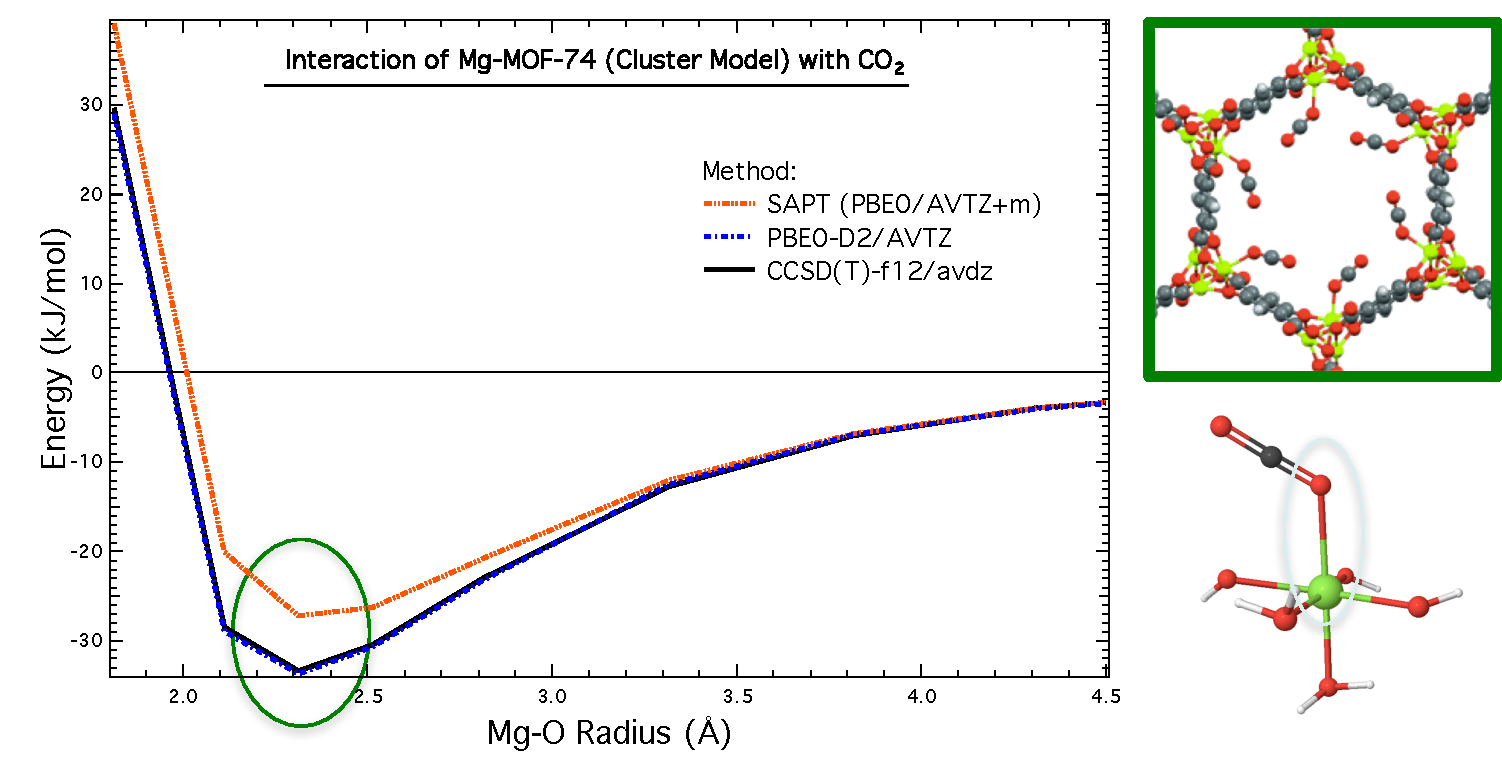
\includegraphics[width=1.0\textwidth]{lmoeda/sapt_breakdown.pdf}
    \caption{
Model \pes for interactions between \co and \mgmof.  (Left) Interaction
energies between \co and a cluster model of \mgmof (shown bottom right),
computed at a \ccsdtf (black), \sapt (orange), and/or \pbeod (blue) level of
theory. Discrepancies
between \sapt and \ccsdtf in the minimum-energy region of the potential have
been highlighted. (Top right)
The structure of \co-bound \mgmof. (Bottom right) The structure of the cluster
model used for \mgmof, where the circled atom pair indicates the relevant Mg-O
radius from the x-axis in the leftmost figure.
            }
    \label{fig:lmoeda-sapt_breakdown}
    \end{figure}
    %%%%%%%%%%%% SAPT Breakdown %%%%%%%%%%%%%%%


In the generation of force fields for \cus-\mofs, we expect that many of the
advantages of the above workflow (such as the component-by-component based
parameterization and method for partial charge determination) will translate
well to force field development for this subclass of \mof materials. 
Nevertheless, there are two reasons why a \sapt-based methodology
cannot be used to generate such force fields. First, and as shown in
\cref{fig:lmoeda-sapt_breakdown} for a representative \mgmof cluster model,
we have empirically found \sapt to be in error compared to benchmark
\ccsdtf calculations. \sapt is well-known to struggle with highly-polarizable
and/or ionic systems, and so this error is perhaps not surprising.
(Possible sources of the discrepancy between \sapt and \ccsdtf will be
discussed in \cref{sec:lmoeda-results}.) Nevertheless, and in the absence of
fortuitous error cancellation,
predictions from an ab initio force field can only be
as good as the
level of theory that they are parameterized against. Consequently, because
\sapt underbinds \co 
by a full \kjmol{6} compared to \ccsdtf, we would not expect to see
good predictions for the \co adsorption isotherm with a \sapt-based
methodology, and a new strategy will be required.

As a second barrier to using a \sapt-based methodology, many of the compounds in the M-\mof-74 series are
open-shell. Though this poses no fundamental issue, 
in practice most implementations of \sapt (aside from the
seldom-used \sapt2012 package developed in Krzysztof Szalewicz's group at
Delaware) do not allow for computations of open-shell systems, and indeed
\sapt-based studies of open-shell compounds are very
rare.\cite{Zuchowski2008a} For these reasons, a new electronic structure
benchmark is highly preferable.

Based on the results for \mgmof, it is clear that, at least for \cus-\mofs, a
new methodology is required which simultaneously keeps the important advantages of the
old workflow (especially the component-by-component based parameterization,
which is essential for generating transferable force fields) while overcoming
the limitations of \sapt itself. Put differently, for \cus-\mofs we should
seek a new electronic structure theory benchmark and associated energy
decomposition analysis with the following qualities:
%
\begin{enumerate}
\item High accuracy with respect to to \ccsdtf benchmark energies
\item Physically-meaningful energy decomposition into (at least)
electrostatics, exchange, induction, and dispersion
\item For systems where \sapt and \ccsdtf agree, a quantitative correspondence
between the energy decompositions of \sapt and the new method
\end{enumerate}
%
Assuming these three qualites are met, we expect to be able to generate force
fields for \cus-\mofs that are both highly accurate and maximally-compatible
with previous force fields developed for coordinatively-saturated \mof
systems. For reasons discussed below, and after a thorough comparison of
available energy decomposition schemes, the \lmoeda\cite{Su2009,Chen2010} has been selected as our
energy decomposition of choice, and we turn now to a full description of the
method and our reasons for using it in this work.

\end{section}


%% =======================
%% 
%% \mgmof has good \co capacity: \cite{Krishna2011}
%% Choice of cluster significantly impacts binding energies: \cite{Getman2012}
%% \co-\mof force field for Cu, Co, Mn, Ni-MOF-74: \cite{Haldoupis2015}
%%     Isotherms are okay (better than UFF, certainly, but still overpredicts
%%     adsorption at high loadings), and would only be applicable to \co adsorption.
%% Another \co-\mof force field for M = Co, Cr, Cu, Fe, Mg, Mn, Ni, Ti, V, and
%% Zn: \cite{Becker2017} 
%%     - Uses UFF (framework) and Trappe (CO2) as starting points, but also
%%     includes polarization. Pretty good agreement between adsorption isotherms. 
%%     - Fit Mg-MOF-74/\co potential to experiment, but then used the same
%%     scaling parameters to compute other M-MOF-74 and CH4 adsorption. Some MOFs and
%%     the CH4 isotherms are not reproduced well, but technically their model isn't
%%     site-specific.
%% "Approaching-paths" non-polarizable \co adsorption model: \cite{Lin2014}
%%     Reproduces Mg and Zn energies, and can be parameterized for both \co and
%%     h2o. Non-polarizable, so the parameters probably don't transfer well to new Mg
%%     environments.
